\documentclass[12pt,letterpaper]{article}
\usepackage[utf8]{inputenc}
\usepackage[spanish]{babel}
\usepackage{times}
\usepackage[left=3cm,top=2.5cm,bottom=2.5cm,right=2.5cm]{geometry}
\usepackage{graphicx}
\title{EV\_ 2\_ 1\_ Diseño\_ del\_ puente\_ H}


\begin{document}
\maketitle




\paragraph{ UNIVERSIDAD POLITÉCNICA DE LA ZONA METROPOLITANA DE GUADALAJARA}

\
\begin{figure}[h!]
\begin{center}


\includegraphics[scale=0.8]{Upzmg.png} 
\label{Upzmg}


\end{center}
\end{figure}


\

\author{Perez Alba Santiago Eduardo. \\ Romero Jauregui Osvaldo.
\

Fecha: 25 de Octubre del 2019.
\

Curso: Sep-Nov 2019.

\
Carrera: Ingeniería en Mecatronica.\

Docente: Moran Garabito Carlos Enrique}

\newpage

\section{Introducción:}
\
Durante la elaboración de esta practica se utilizaran circuitos vistos anteriormente, como por ejemplo el de los relevadores y los optoacopladores junto con la placa de arduino, se retomaran conceptos de los mismos e incluirán nuevos como lo es el funcionamiento de los MOSFET. Durante su desarrollo se podrá ver el funcionamiento de cada uno de ellos para cumplir el objetivo de la practica.

\section{Objetivo:}
\
Lograr el cambio de giro de nuestro motor DC, de tal manera que, al presionar uno de los push buttons haga el giro hacia un lado, y al presionar el otro, gire al lado contrario,

\section{Materiales:}
\
\begin{itemize}
\item Protoboard
\item 4n25 OptoAcopladores
\item Jumpers
\item Relevadores
\item Mosfet IRF640N
\item Resistencias Varias
\item Fuente DC
\item Clavija a CA
\item Motor DC
\end{itemize}
\
\section{Marco teórico:}
\
\textbf{Motor:} El motor de corriente continua (motor DC) es una maquina que convierte la energía eléctrica en mecánica, provocando un movimiento rotatorio. En algunas modificaciones, ejercen tracción sobre un riel. Estos motores se conocen como motores lineales.

\
Una maquina de corriente continua (generador o motor) se compone principalmente de dos partes, un estator que da soporte mecánico al aparato y tiene un hueco en el centro generalmente de forma cilíndrica. En el estator ademas se encuentran los polos, que pueden ser de imanes permanentes o devanados con hilo de cobre sobre el núcleo de hierro. El rotor es generalmente de forma cilíndrica, también devanado y con núcleo, al que llega la corriente mediante dos escobillas.
\
\textbf{Puente H:} El puente H es un circuito electronico que permite a un motor eléctrico DC girar en ambos sentidos, avanzar y retroceder. Los puentes H ya vienen hechos en algunos circuitos integrados, pero también se pueden construir a partir de componentes eléctricos y/o electrónicos. Un puente H se construye con 4 interruptores (mecánicos o mediante transistores). Cuando los interruptores S1 y S4 están cerrados (S2 y S3 abiertos ) se aplica una tension haciendo girar el motor en un sentido. Abriendo los interruptores S1 y S4(cerrando S2 y S3), el voltaje se invierte permitiendo el giro en sentido inverso del motor.

\begin{figure}[h!]
\begin{center}
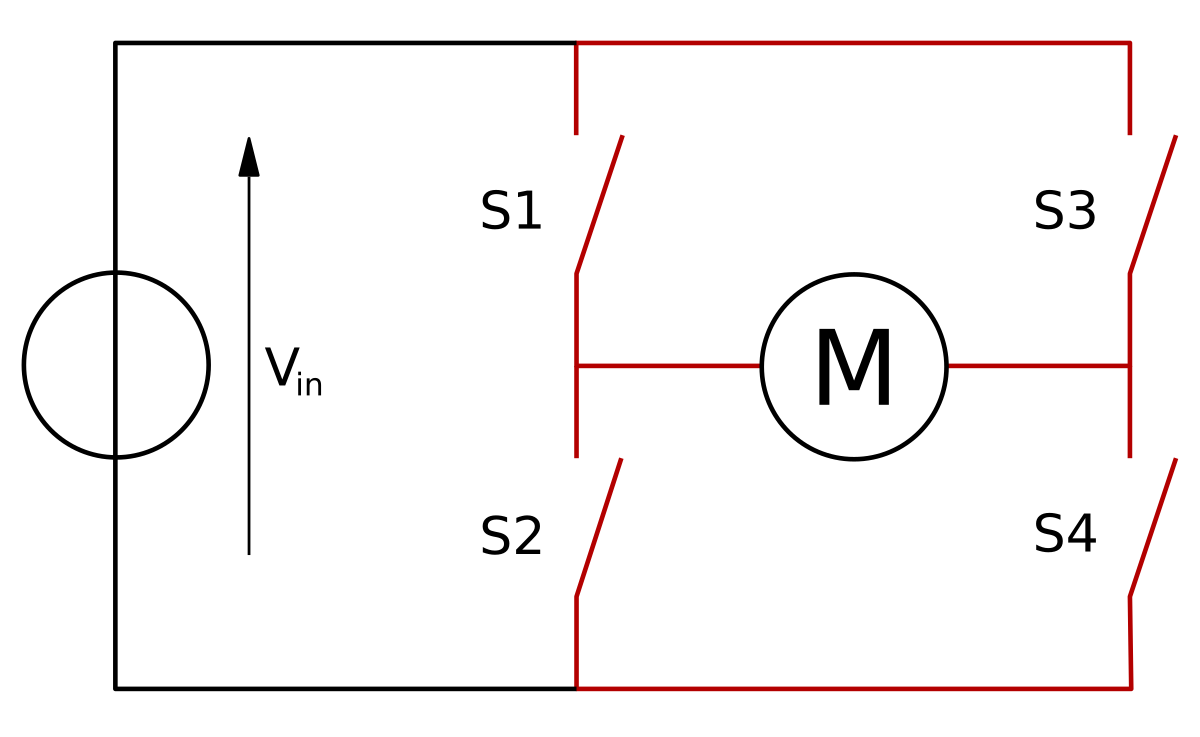
\includegraphics[scale=0.1]{PuenteHR.png}
\caption{Puente H.}
\end{center}
\end{figure}

\section{Procedimiento:}

\
\begin{itemize}
\item Primeramente revisaremos el circuito complementario otorgado por el maestro.

\
\begin{figure}[h!]
\begin{center}
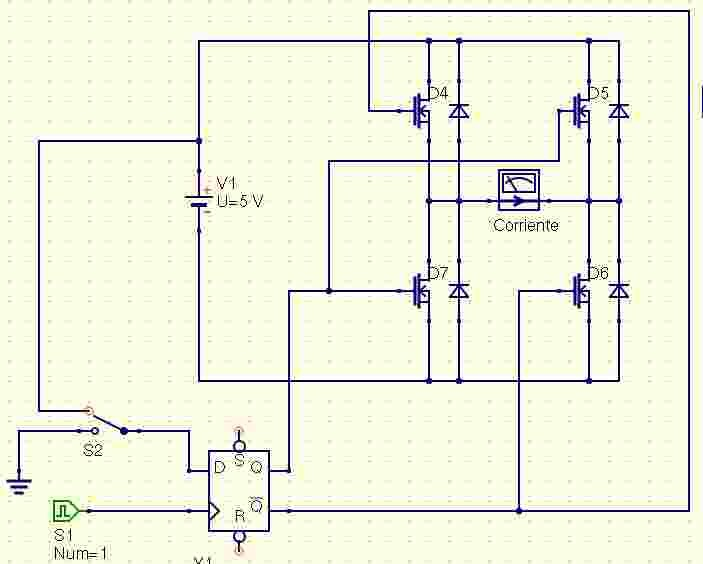
\includegraphics[scale=0.5]{PuenteH.jpg}
\caption{Puente H-Practica.}
\end{center}
\end{figure}

\item Luego se procederá a añadir este circuito complementario al circuito realizado en la practica 2.

\
\begin{figure}[h!]
\begin{center}
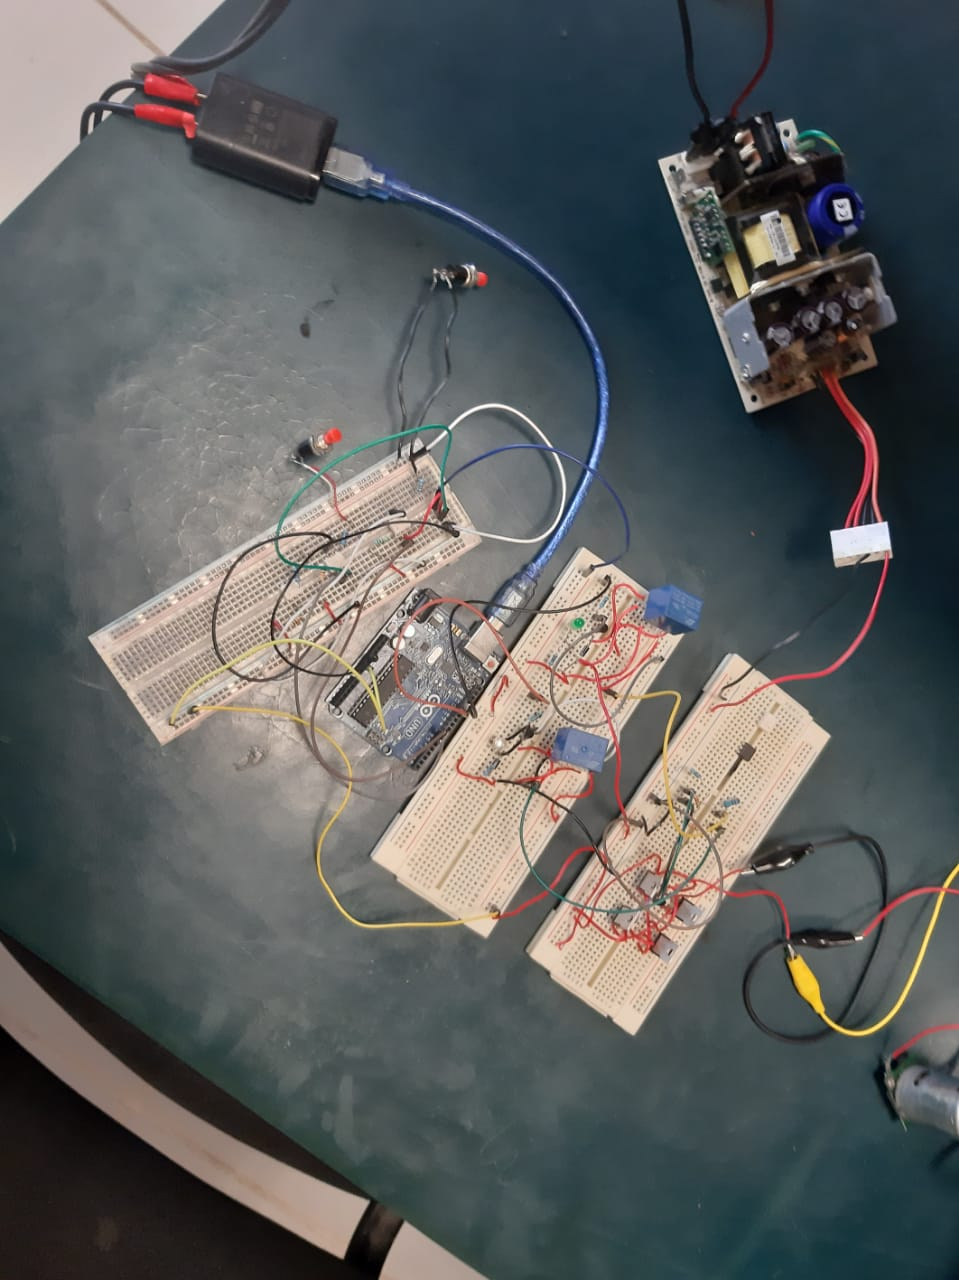
\includegraphics[scale=0.2]{Circuito1.jpeg}

\caption{Puente H-Circuito.}
\end{center}
\end{figure}

\newpage
\item Conectaremos nuestro motor y nuestras fuentes, logrando hacer funcionar nuestro puente H.
En el cual el puente H deberían ir en paralelo, y conectar cruzada o en forma de "x" la \textbf{Gate-Gate} con los mosfet 1-4, y nuevamente hacerlo con los mosfet 2-3, luego de eso conectar \textbf{Source-Source} respectivamente del mosfet 1-3, para después conectar \textbf{Drain-Drain} respectivamente del mosfet 2-4, Ahora conectaremos del \textbf{Source-Tierra} respectivamente de nuestra fuente(Todas las tierras comunes), y por ultimo conectaremos \textbf{Drain-Positivo} respectivamente de la entrada de nuestra fuente.

\
\begin{figure}[h!]
\begin{center}
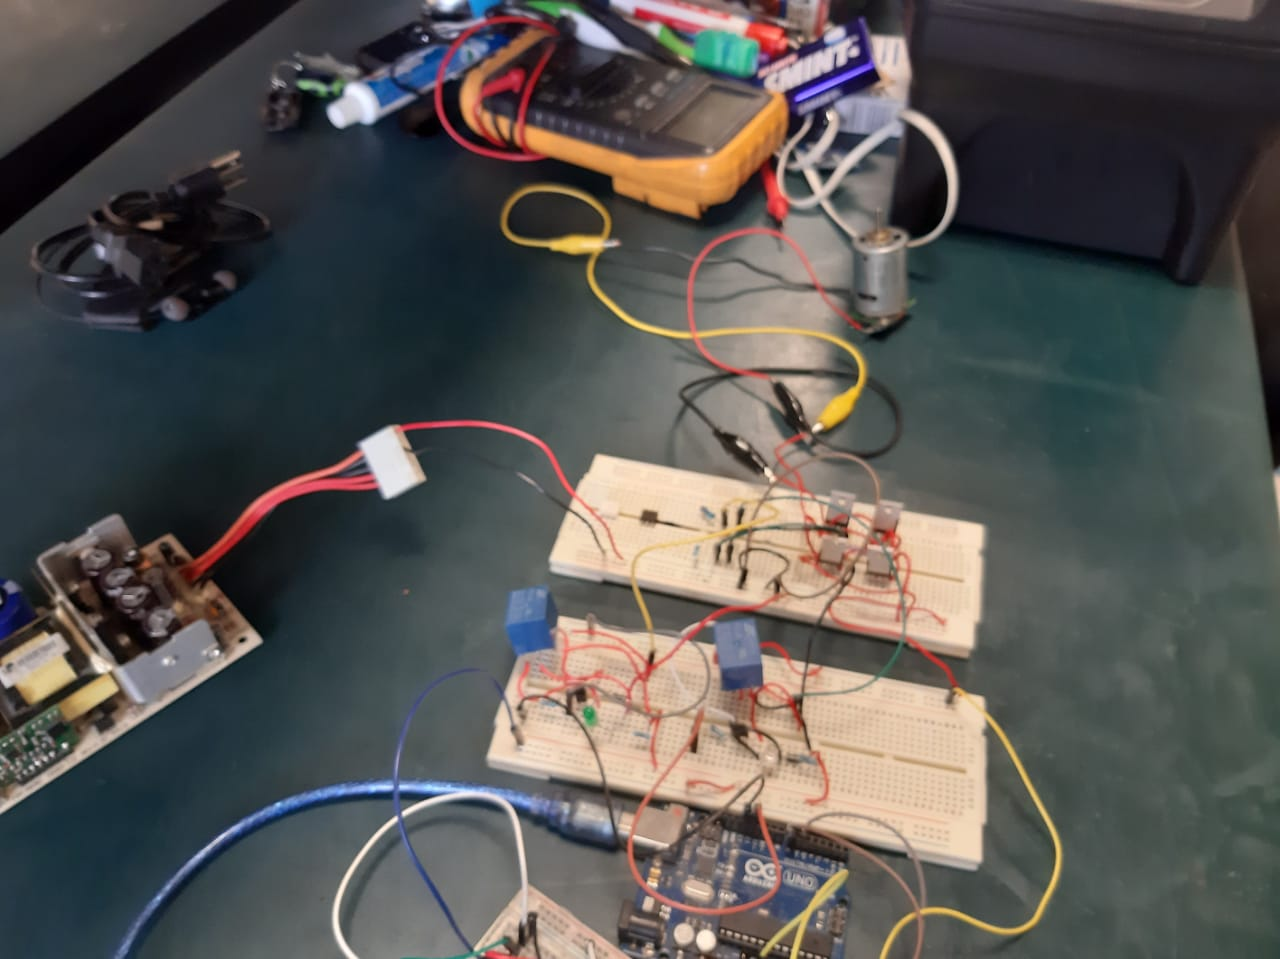
\includegraphics[scale=0.2]{Circuito2.jpeg}

\caption{Puente H-Armado}
\end{center}
\end{figure}
\end{itemize}

\section{Conclusión:}
\begin{itemize}

\item Durante la elaboración de esta practica se encontraron ciertas dificultades en las conexiones de los MOSFET, debido a la errónea colocación y situado de nuestras GATE, lo cual nos provocaba un calentamiento impropio de los MOSFET, y el mal funcionamiento del circuito en complemento, al momento de revisar nuevamente las conexión y volver a conectar de manera adecuada y con cuerdo al Data Sheet de nuestro material logramos el correcto funcionamiento, en el cual se mostraba el giro en ambos sentidos con la presión de sus respectivos botones.
\item  Durante la elaboración de la practica nos encontramos con un mal funcionamiento de los MOSFET, esto debido a que teníamos una mala conexión entre GATE, ya que conectamos en serie dos mosfet, por lo cual no nos creaba el flujo de la corriente y no nos accionaba el motor, sin dejar de lado que se comenzaba el sobrecalentamiento del mosfet. Una vez revisada la conexión de la manera correcta se accionaba el motor hacia ambos sentidos sin ningún problema, asi cumpliendo nuestro objetivo
\end{itemize}

\end{document}